\chapter{Quaternion graph signal processing}
\label{ch:QGSP}

Graph signal processing is a highly flexible tool for analysing and transforming graph-based data. However, as it happens with so many engineering tasks, often it appears to mix mathematics and art: the experienced GSP user knows that quite a few characteristics of the underlying graph are open to be determined by the very problem at hand and by the user's intuition. That is, whether one must consider real or complex edge weights, directed or undirected graphs, whether loops or multiple edges shall be allowed, all of these modeling choices arise from the data and from the way one considers the most appropriate to represent the relations within. We make hereby the argument that changing the algebra over which the graph signal samples (and edge weights) are defined, although rarely regarded among modeling choices, may reveal powerful new tools.

Let us take an example of how the signal algebra may affect the processing possibilities, in the current state of GSP. Undirected graphs with real-valued weights are a common option for those used to model data defined over geographic spaces, since it is reasonable to consider the adjacency relations to be non-directional and weighted by positive real numbers \cite{shuman2013emerging}. However, the same topology would be arguably inappropriate should one deal with complex-valued signals: a directed graph or a graph with complex-valued edge weights would be more reasonable options to evaluate, since they would produce graph Fourier transform matrices with complex entries. Although this scenario may seem to lack practical purpose, defining a graph signal with samples lying in extensions of the real field (e.g. complex numbers) would be justified by the increase in the amount of information stored within each sample (from a single real number, to twice as much in the complex case).

Electrical engineers for many decades have exploited the benefits of handling more than one real-valued information (e.g. magnitude and phase) encoded in a single signal sample, and a similar motivation led to Sangwine's \cite{sangwine1996fourier} discrete version of a family of bidimensional transforms over the \textit{quaternions} (a skew-field which extends the complex numbers by having four real valued components). As the reader may recall from Chapter \ref{ch:Intro}, these transforms used this class of hypercomplex numbers to perform holistic color image processing, handling all three color channels at once. In fact, \emph{quaternion signal processing} was created to embed three- or four-dimensional data into one-dimensional signals \cite{took2008quaternion}. Ever since, quaternion transforms have been employed not only on color image processing \cite{ell2007hypercomplex,chen2018quaternion,li2013quaternion,evans2000hypercomplex}, but also on other tasks such as bivariate signal analysis \cite{flamant2017spectral,flamant2017time,flamant2018complete}.

In Chapter \ref{ch:reviewGSP} it was presented the motivation and fundamentals of graph signal processing, while Chapter \ref{ch:FrGSO} delved into the exploration of a fractional graph shift.
This chapter attempts to further extend the borders of GSP by pondering the problem of signal processing on graphs with quaternion-valued edge weights, referred to as \textit{quaternion graph signal processing}.

\section{Laying the foundations for QGSP}

Since QGSP is the development and application of GSP tools to the context of quaternion-valued signals and graph edge weights, it starts by extending the usual definition of graph signal in (\ref{eq:def_signal}), replacing the complex-valued numbers with quaternions. As such, the quaternion graph signal $\mathbf{s}$, defined over the graph $\mathcal{G} = \{\mathcal{V}, \mathbf{A}\}  \ | \ \mathbf{A} \in \mathbb{H}^{n \times n}$, is defined as
\begin{equation}\label{eq:qgsp_defs}
    s: \ \mathcal{V} \rightarrow \mathbb{H} \ | \ s(v_i) = s_i.
\end{equation}

This definition unfolds some challenges: what does it
mean to have a smooth quaternion graph signal? Does the well known benefit of quaternion signal processing, namely holistic manipulation of multiple channels of information, transfer to graph signal processing? How is one able to design LSI filters in QGSP?

In order to properly address these questions and establish the foundations of QGSP, a few milestones were set to be conquered. Firstly, an algorithm to compute the direct and inverse (quaternion) graph Fourier transforms should be proposed, to allow for basic spectral analysis. This includes revisiting the definition of frequency ordering, which is well understood only for real and complex graph signals. Secondly, QGSP should ideally provide a class of graphs for which the Fourier transform is known to exist (and hopefully easier to compute than outside this class). The reasoning here is to find a case similar to that of usual GSP, where it is known that undirected graphs with real-valued edge weights always have diagonalizable GSOs. Finally, QGSP should ideally provide a method to design graph FIR filters, tailored to approximate a given frequency response. The Subsection \ref{subsec:eigendecomposition} gives the first step towards QGSP, properly defining the QGFT and studying the eigendecomposition of the quaternion graph shift operator (QGSO).

\subsection{Eigendecomposing the shift operator}
\label{subsec:eigendecomposition}
At the very center of vertex-frequency analysis in GSP lies the definition that a basis of eigenvectors of the chosen graph shift operator act as Fourier components for the space of graph signals. This can be directly translated to QGSP, after taking into account the results presented in Chapter \ref{ch:reviewQuat}, regarding diagonalization of quaternion matrices.

\begin{definition}
    Given the graph $\mathcal{G} = \{\mathcal{V}, \mathbf{A}\}  $,  with adjacency matrix $ \mathbf{A} \in \mathbb{H}^{n \times n}$, the \textit{quaternion graph Fourier transform} (QGFT) is the projection of a graph signal onto the eigenspace of $\mathbf{A}$.
\end{definition}

The first step towards the QGFT is, therefore, the generation of a basis of (possibly generalized) eigenvectors of the adjacency matrix. This work has dealt only with the case of diagonalizable graph matrices, but the use of the Jordan canonical form can be investigated for non-diagonalizable QGSOs \cite{Longxuan1996}.

On the one hand, from the Corollary \ref{cor:diagonalizable} it is known that the diagonalizability of an adjacency matrix $\mathbf{A}$ both implies and requires that of its complex adjoint matrix $\rchi_A$. Let us write $\mathbf{A} = \mathbf{V} \mathbf{\Lambda} \mathbf{V}^{-1}$. On the other hand, Theorem \ref{th:02} guarantees that the eigenvalues of the adjacency matrix can be taken as half the ones of its complex adjoint matrix. More specifically, they can be taken as the union of the set of eigenvalues with positive imaginary part (recall that they are complex-valued) and the set of \textit{distinct} eigenvalues with null imaginary part (recall that every real-valued eigenvalue appears twice).

However, once the desired eigenvalues from $\rchi_A$ have been defined, how does one assemble $\mathbf{V}$ out of the eigenvectors of $\rchi_A$? That is answered by Equation (\ref{eq:eigvalueequation}), which is rewritten below for convenience:
\begin{equation*}
    \begin{pmatrix}
        \mathbf{A}_1              & \mathbf{A}_2            \\
        - \overline{\mathbf{A}}_2 & \overline{\mathbf{A}}_1
    \end{pmatrix}
    \begin{pmatrix}
        \mathbf{v}_1 \\
        - \overline{\mathbf{v}}_2
    \end{pmatrix} =
    \begin{pmatrix}
        \mathbf{v}_1 \\
        - \overline{\mathbf{v}}_2
    \end{pmatrix}
    \lambda.
\end{equation*}
On the left-hand side of the equation, we find $\rchi_A$ and one of its eigenvectors, which is written in terms of the symplectic decomposition of a quaternionic column vector $\mathbf{v} = \mathbf{v}_1 + \mathbf{v}_2 \qj$. As it turns out, $\mathbf{v}$ is precisely the eigenvector of $\mathbf{A}$ associated with the eigenvalue $\lambda$. This is proven in Appendix \ref{ch:AppendixA} and constitutes a minor contribution of this thesis. The answer to the question raised a few lines above, to sum up, is that once one has the chosen eigenvalues of $\rchi_A$, it is possible to assemble $\mathbf{V} \in \mathbb{H}^{n \times n}$ out of the respective eigenvectors of $\rchi_A$ by simply spliting these $2n$-long eigenvectors into halves: the first half corresponds to $\mathbf{v}_1$ (the simplex part of the eigenvector $\mathbf{v}$), while the second half is $- \overline{\mathbf{v}}_2$ (with $\mathbf{v}_2$ being the perplex part of $\mathbf{v}$).

So far we are able to obtain $\mathbf{V}$ from $\mathbf{A}$, bypassing the direct eigendecomposition of a quaternion matrix by using its complex adjoint. However, the question of how to get $\mathbf{V}^{-1}$, if it exists, poses itself imediately, after all $\mathbf{V}$ corresponds to the \textit{inverse} of the QGFT. Let us address this point.

\subsection{Inversion of the eigenvector matrix and frequency ordering}
\label{subsec:inversion}
The inversion of quaternion matrices is certainly a problem tackled by many researchers, but is not featured prominently in literature, at least not as far as the author is aware. There is, however, an algorithm proposed by \cite{cohen1999quaternionic} during studies on the determinant of quaternion matrices, when they highlighted the utility of Schur complements on computing the inversion of any matrix $\mathbf{M} \in \mathcal{R}^{n \times n}$ over the ring $\mathcal{R}$. Let us go quickly through their idea. Given that $\mathbf{M}$ is written in block form,
\begin{equation}
    \label{eq:block}
    \mathbf{M} = \begin{pmatrix}
        \mathbf{A} & \mathbf{B} \\
        \mathbf{C} & \mathbf{D}
    \end{pmatrix},
\end{equation}
and under the requisite that $\mathbf{A} \in \mathcal{R}^{k \times k}$ is invertible, the Schur complement of $\mathbf{A}$ in $\mathbf{M}$ is defined as
\begin{equation}
    \mathbf{A}_s \overset{\Delta}{=} \mathbf{D}
    - \mathbf{C}\mathbf{A}^{-1} \mathbf{B}.
\end{equation}
Given that $\mathbf{A}_s$ is also invertible, the closed formula for the inverse of $\mathbf{M}$ is
\begin{equation}
    \label{eq:schur}
    \mathbf{M}^{-1} =
    \begin{pmatrix}
        \mathbf{I}_k & - \mathbf{A}^{-1} \mathbf{B} \\
        \mathbf{0}   & \mathbf{I}_{n - k}
    \end{pmatrix}
    \begin{pmatrix}
        \mathbf{A}^{-1} & \mathbf{0}        \\
        \mathbf{0}      & \mathbf{A}_s^{-1}
    \end{pmatrix}
    \begin{pmatrix}
        \mathbf{I}_k                 & \mathbf{0}         \\
        - \mathbf{C} \mathbf{A}^{-1} & \mathbf{I}_{n - k}
    \end{pmatrix},
\end{equation}
so that the inversion of $\mathbf{M}$ is now reduced to inversion of the two smaller matrices $\mathbf{A}$ and $\mathbf{A}_s$.

Although this method proposes a closed formula for quaternion matrix inversion, it requires an exhaustive search for a submatrix in the upper left corner that, simultaneously, is \textit{invertible} and \textit{has invertible Schur complement}. Probably the idea can be explored in the future and used to find an efficient way to compute $\mathbf{V}^{-1}$, but in Algorithm \ref{alg:qinv} we propose a more reasonable compromise between processing speed, implementation time and broad applicability.

The reasoning goes as follows. According to Theorem \ref{th:equiv02}, a necessary and sufficient condition for the invertibility of a matrix $\mathbf{V} \in \mathbb{H}^{n \times n}$ is the existance of $\rchi^{-1}_{V}$. Moreover, from Theorem \ref{th:equiv01}, if $\rchi^{-1}_{V}$ exists and has the form of a complex adjoint matrix, let us say $\rchi_{V}^{-1} = \rchi_{M}$, then it follows that $\mathbf{M} = \mathbf{V}^{-1}$, since the theorem guarantees that
\begin{equation}
    \rchi_{V} \rchi_{M} = \rchi_{V} \rchi_{V}^{-1} = \mathbf{I}_{2n \times 2n} = \rchi_{I_{n \times n}}
    \Rightarrow \mathbf{V} \mathbf{M} = \mathbf{I}_{n \times n},
\end{equation}
letting $\mathbf{I}_{m \times m}$ be the identity matrix of order $m$.\footnote{For simplicity, this notation is slightly loose, representing both a complex- and a quaternion-valued identity matrix, since in both cases their entries have zero-valued or zero-normed imaginary parts.} That is, once the complex adjoint of $\mathbf{V}$ is computed, one simply needs to compute its inverse, if it exists, and verify if it follows the format in Definition \ref{def:complexadjoint}.

\newcommand{\algorithmspacing}{0.5}
\begin{algorithm}
    \label{alg:qinv}
    Compute the inverse of a quaternion-valued matrix, if a sufficient condition for its existence is met:
    \vspace*{-\algorithmspacing\baselineskip}
    \begin{leftbar}
        \noindent\textbf{\upshape Input:} $\mathbf{V} \in \mathbb{H}^{n \times n}$. \textbf{\upshape Output:} $\mathbf{V}^{-1}$ or {\upshape None}.

        \begin{algorithmic}[1]
            \State $\rchi_V \gets \mathrm{to\_complex\_adjoint}(\mathbf{V})$
            \If{$\det(\rchi_V) = 0$}
            \State \Return {\upshape None}
            \Else
            \State $\mathbf{U} \gets \mathrm{inverse}(\rchi_V)$
            \If{$\mathbf{not} \ \mathrm{has\_complex\_adjoint\_form}(\mathbf{U})$}
            \State \Return {\upshape None}
            \Else
            \State $\mathbf{V}^{-1} \gets \mathrm{from\_complex\_adjoint}(\mathbf{U})$
            \State \Return $\mathbf{V}^{-1}$
            \EndIf
            \EndIf
        \end{algorithmic}
    \end{leftbar}
    \vspace*{-\algorithmspacing\baselineskip}
    \noindent These functions were used in the algorithm to improve readability:
    \vspace*{-\algorithmspacing\baselineskip}
    \begin{itemize}[noitemsep]
        \item $\mathrm{to\_complex\_adjoint}$: converts a quaternion matrix to its complex adjoint form.
        \item $\mathrm{from\_complex\_adjoint}$: converts a complex adjoint matrix to its quaternion-valued form.
        \item $\mathrm{inverse}$: computes the inverse of a complex-valued matrix.
        \item $\mathrm{has\_complex\_adjoint\_form}$: checks if the matrix has the complex adjoint form, i.~e., is a block matrix as the one in Definition \ref{def:complexadjoint}.
    \end{itemize}
\end{algorithm}

At this point, all steps required to generate the QGFT, assuming the graph adjacency matrix is diagonalizable, have been addressed. However, the transform still remains of little use until a clear definition of frequency ordering is presented, otherwise the lack of sense of low and high frequencies make the signal spectrum meaningless.

Since the quaternions form a normed algebra --- and the reader may refer back to (\ref{eq:modulusq}) --- it is natural to borrow from classical GSP the definition of the graph total variation as a \textit{metric} for frequency. In fact, even the elegant property of frequency ordering in the complex plane follows from GSP to QGSP. Let us see why.

Let $ \mathbf{A} \in \mathbb{H}^{n \times n}$ be diagonalizable, with standard eigenvalues ordered like so
\begin{equation}
    \label{eq:eig_order_q}
    |\lambda_0| \leq |\lambda_1| \leq \dots \leq |\lambda_{N-1}| \overset{\Delta}{=} |\lambda_{max}|,
\end{equation}
associated with the eigenvectors $ (\mathbf{v}_i)_{i=0,\dots,n-1} $.
Now, let us notice that the graph total variation, defined in (\ref{eq:tv_graphs}), does not have to use $ \ell_1 $-norm for it to quantify the notion of frequency. In fact, let us use the general $ \ell_p $-norm for a moment, with $p \geq 1$, represented as $ \Vert \mathbf{v}\Vert_p \overset{\Delta}{=} \left(\sum_{k=0}^{n-1} |v_k|^p\right)^{1/p} $, for $\mathbf{v} \in \mathbb{H}^n$, and define the graph total variation of the graph signal $\mathbf{s}$ as
\begin{equation}
    \label{eq:tv_graphsq}
    TV_{G, p}(\mathbf{s}) \overset{\Delta}{=} \left\Vert \mathbf{s} - \frac{1}{|\lambda_{max}|}\mathbf{A} \mathbf{s} \right\Vert_p.
\end{equation}

If we take the important step of scaling the eigenvectors $\mathbf{v}_i$ so they have unit $\ell_p$-norm, i.~e., making $\Vert \mathbf{v}_i\Vert_p = 1$, then the associative and distributive properties of quaternion multiplication allow us to do

\begin{equation}
    \begin{aligned}
        TV_{G, p}(\mathbf{v}_k) & =
        \left\Vert \mathbf{v}_k - \frac{1}{|\lambda_{max}|} \mathbf{A} \mathbf{v}_k \right\Vert_p =
        \left\Vert\mathbf{v}_k - \mathbf{v}_k \frac{1}{|\lambda_{max}|} \lambda_k \right\Vert_p                                  \\
                                & = \left\Vert\mathbf{v}_k \left( 1 -  \frac{1}{|\lambda_{max}|} \lambda_k \right) \right\Vert_p \\
                                & =
        \underbrace{\Vert \mathbf{v}_k \Vert_p}_{= 1} \left|1 - \frac{\lambda_k}{|\lambda_{max}|}\right| = \Big| \lambda_k - |\lambda_{max}| \Big| \frac{1}{|\lambda_{max}|}.
    \end{aligned}
\end{equation}
% Since $(1 -  \nicefrac{1}{|\lambda_{max}|} \lambda_k)$ is just a constant complex factor that multiplies each entry in the vector $\mathbf{v}_k$, its modulus may be taken out of the sum in the $\ell_p$-norm computation,
What leads to exactly the same frequency ordering obtained in the classical GSP derivation,
\begin{equation}
    \label{eq:TV_ordering_q}
    \Big| \! \lambda_i  - \! |\lambda_{max}|\Big| \! \leq \! \Big|  \lambda_j  - \! |\lambda_{max}|\Big| \! \! \iff \! \! TV_{G, p}(\mathbf{v}_i) \leq TV_{G, p}(\mathbf{v}_j).
\end{equation}

In other words, once the eigenvectors are individually \textit{normalized}, i.~e., scaled to have unit $\ell_p$-norm, then the farther an eigenvalue lies from the point $|\lambda_{max}|$ in the real line of the complex plane, the greater is its eigenvector graph total variation $TV_{G, p}$. By definition, it means the greater is the frequency it represents. Besides, notice how the scaling implies that the value of $TV_{G, p}$ depends solely on the eigenvalues, not on $p$.

In order to interpret the spectrum domain, the eigenvalues are sorted in ascending order of their respective eigenvector total variation: this sorts the frequency from lowest to highest. When not explicitly mentioned, it is assumed a value of $p = 1$ for all occurrences of $\ell_p$-norm.

\subsection{On the existence of a class of graphs with diagonalizable adjacency matrix}

A relevant topic of discussion, when laying the foundations for QGSP, is to ponder the question on the existence of a class of graphs with diagonalizable QGSOs. It is a reasonable point of investigation, since in classical GSP one can confidently take advantage of some classes of graphs to make sure the shift operator is diagonalizable beforehand, which saves time and effort. Some examples are undirected real-weighted graphs and directed ring graphs with equal edge weights.

The reader may notice that undirected quaternion graphs do not possess necessarily a diagonalizable adjacency matrix. Indeed, the fact that $\mathbf{A}$ is symmetric has no effect on proving the diagonalizability of its complex adjoint,
\begin{equation}
    \begin{pmatrix}
        \mathbf{A}_1              & \mathbf{A}_2            \\
        - \overline{\mathbf{A}}_2 & \overline{\mathbf{A}}_1
    \end{pmatrix}.
\end{equation}

The subjacent reason as to why undirected real-weighted graphs have diagonalizable adjacency matrices is that these real-valued matrices are symmetric, or more generally \textit{normal}, i.~e., they commute with (because are equal to) their transpose. In the case of complex-valued matrices, being normal (i.~e., commuting with their Hermitian transpose) also suffices for proving their diagonalizability. So, in order to find quaternion graphs analogous to undirected real-weighted graphs, in the sense of having a sufficient condition for diagonalizable shift operators, their adjacency matrix must possess \textit{normal} complex adjoint matrices. Fortunately, Theorem \ref{th:equiv01} states the condition:
$ \rchi_{A}$ is normal ($ \rchi_{A}^H \rchi_{A} = \rchi_{A} \rchi_{A}^H $) or Hermitian ($\rchi_{A}^H = \rchi_{A}$) if and only if so is $ \mathbf{A}$.

Zhang claims Theorem \ref{th:equiv01} is proved by direct verification \cite{zhang1997quaternions}, but let us go through a way to visualize part of the proof within the context of GSP.

\begin{proof}
    The part of the Theorem about to be verified is: \emph{is it true that Hermitian quaternion-valued matrices have Hermitian complex adjoints?} Equivalently,
    \begin{equation}
        \mathbf{A}^H = \mathbf{A}, \ \mathbf{A} \in \mathbb{H}^{n \times n} \Rightarrow
        \rchi_{A}^H = \rchi_{A}, \ \rchi_{A} \in \mathbb{C}^{2n \times 2n}?
    \end{equation}

    Look at $\mathbf{A}$ as a graph adjacency matrix and let $A_{i,j} = a + b\qi + c\qj + d\qk$ be the weight of the edge going from $v_j$ to $v_i$. The hypothesis of a Hermitian quaternion-valued matrix implies $A_{j,i} = \overline{A_{i,j}}$, or $A_{j,i} = a - b\qi - c\qj - d\qk$. As an example, a pair of connected vertices in this graph is represented in Fig. \ref{fig:hermitian-crop-2}, in which one can see the edges in opposite directions and with conjugate edge weights.

    Fig. \ref{fig:hermitian-crop-2} depicts also the edges that would arise separately from the simplex and perplex parts of the edge weights (see the center and right diagrams). For instance, the edge weight $A_{j,i} = a - b\qi - c\qj - d\qk$ satisfies\footnote{Notice how the notation will mix once more in this thesis the superscripts \textsuperscript{(s)} and \textsuperscript{(p)} along with the subscripts 1 and 2 to indicate the symplectic decomposition parts.}
    \begin{equation}
        A_{j,i} = A^{(s)}_{j,i} + A^{(p)}_{j,i} \qj, \text{ with }
        \begin{cases}
            A^{(s)}_{j,i} = a - b\qi \\
            A^{(p)}_{j,i} = -c -d \qi
        \end{cases}.
    \end{equation}

    \begin{figure}
        \centering
        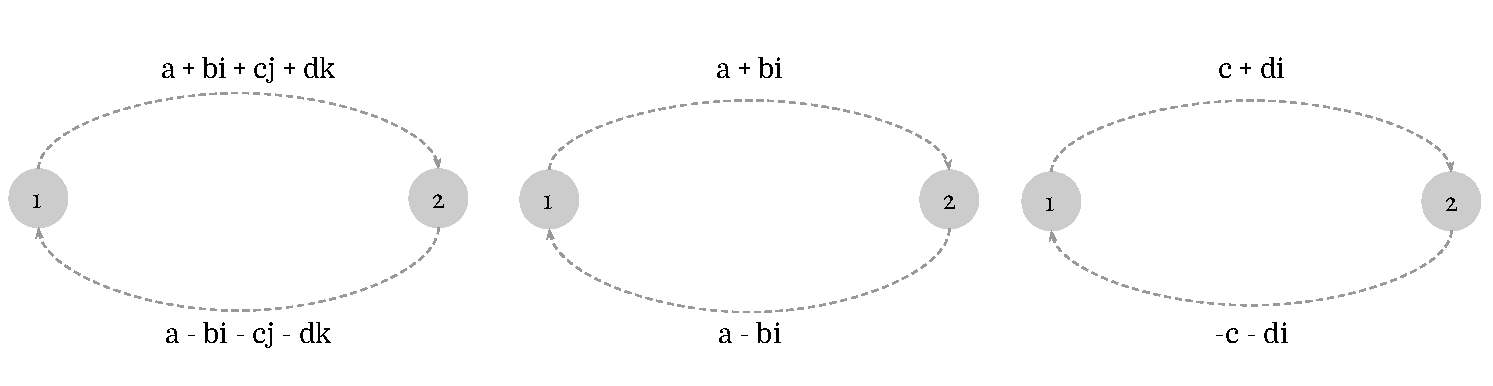
\includegraphics[width=0.95\linewidth]{Figures/hermitian-crop-2.pdf}
        \caption{Illustration of two connected vertices in a graph with Hermitian adjacency matrix (left-hand side). In the center and on the right, respectively, are displayed the edges created by the simplex and perplex parts of the adjacency matrix.}
        \label{fig:hermitian-crop-2}
    \end{figure}

    This (along with Fig. \ref{fig:hermitian-crop-2}) sheds light on the symplectic decomposition of $\mathbf{A}$: its symplex part satisfies $\mathbf{A}^T_1 = \overline{\mathbf{A}_1}$ (complex Hermitian matrix) while its perplex satisfies $\mathbf{A}^T_2 = - \mathbf{A}_2$.
    With this in mind, the Hermitian of the complex adjoint yields
    \begin{equation}
        \rchi_A^H =
        \begin{pmatrix}
            \mathbf{A}^H_1 & - \mathbf{A}^T_2 \\
            \mathbf{A}^H_2 & \mathbf{A}^T_1
        \end{pmatrix}
        =
        \begin{pmatrix}
            \mathbf{A}_1             & \mathbf{A}_2            \\
            -\overline{\mathbf{A}}_2 & \overline{\mathbf{A}}_1
        \end{pmatrix},
    \end{equation}
    precisely the matrix $\rchi_A$, as intended to be proved.
\end{proof}

\subsection{Does a Hermitian QGSO have unitary eigenvector matrix?}

It is known that every Hermitian complex matrix is diagonalizable by a unitary matrix and has only real-valued eigenvalues. In other words, if $\mathbf{M} \in \mathbb{C}^{n \times n}$ and $\mathbf{M} = \mathbf{M}^H$, then there exists a complex matrix $\mathbf{U}$ and a diagonal real matrix $\mathbf{\Gamma}$ so that $\mathbf{M} = \mathbf{U} \mathbf{\Gamma} \mathbf{U}^{-1}$ and $\mathbf{U}^{-1} = \mathbf{U}^H$. However, despite the fact one can guarantee that a Hermitian QGSO has a Hermitian complex adjoint matrix, one could ponder the question whether this implies its eigenvector matrix is necessarily unitary. Let us verify this.

Let $\mathbf{A}$ be a Hermitian (hence diagonalizable) quaternion adjacency matrix, therefore $\mathbf{A} \mathbf{V} = \mathbf{V} \mathbf{\Lambda}$. Since $\rchi_{A}$ is complex-valued and Hermitian, its eigenvector matrix (let us say, $\mathbf{\Phi}$) is unitary and we may write $\rchi_{A} = \mathbf{\Phi} \mathbf{\Gamma} \mathbf{\Phi}^H$. Each column $\qphi$ in $\mathbf{\Phi}$, the reader may recall, is written is terms of the simplex and perplex parts (which are complex-valued) of the respective column $\mathbf{v}$ in $\mathbf{V}$:
\begin{equation}
    \mathbf{\qphi}^{(n)} =
    \begin{pmatrix}
        \mathbf{v}^{(n)}_1 \\
        - \overline{\mathbf{v}}^{(n)}_2
    \end{pmatrix}.
\end{equation}

Since $\mathbf{\Phi}$ is unitary,
\begin{equation}
    \label{eq:phi_hermitian}
    \begin{aligned}
        {\mathbf{\qphi}^{(n)}}^H \mathbf{\qphi}^{(n)} = 1 \\
        \Big({\mathbf{v}^{(n)}_1}^H \quad - {\mathbf{v}^{(n)}_2}^T \Big)
        \begin{pmatrix}
            \mathbf{v}^{(n)}_1 \\
            - \overline{\mathbf{v}}^{(n)}_2
        \end{pmatrix} = 1       \\
        {\mathbf{v}^{(n)}_1}^H \mathbf{v}^{(n)}_1 + {\mathbf{v}^{(n)}_2}^T \overline{\mathbf{v}}^{(n)}_2 = 1.
    \end{aligned}
\end{equation}
Now, does the final equality in (\ref{eq:phi_hermitian}) imply that ${\mathbf{v}^{(n)}}^H \mathbf{v}^{(n)} = 1$? If so, this would make the quaternion-valued eigenvector matrix $\mathbf{V}$ unitary. Let us drop the superscript $n$ temporarily, to clean the notation during the following lines. Since $\mathbf{v} = \mathbf{v}_1 + \mathbf{v}_2 \qj$,
\begin{equation}
    \begin{aligned}
        \mathbf{v}^H \mathbf{v} & = (\mathbf{v}^H_1 - \mathbf{v}^T_2 \qj) (\mathbf{v}_1 + \mathbf{v}_2 \qj)                                                                                       \\
                                & = \mathbf{v}^H_1 \mathbf{v}_1 + \mathbf{v}^H_1 \mathbf{v}_2 \qj
        - \underbrace{\mathbf{v}^T_2 \qj \mathbf{v}_1}_{\mathbf{v}^T_2 \overline{\mathbf{v}}_1 \qj} - \underbrace{\mathbf{v}_2^T \qj \mathbf{v}_2 \qj}_{- \mathbf{v}_2^T \overline{\mathbf{v}}_2} \\
                                & = \underbrace{\mathbf{v}_1^H \mathbf{v}_1 + \mathbf{v}_2^T \overline{\mathbf{v}}_2}_{= 1} +
        (\mathbf{v}^H_1 \mathbf{v}_2 - \mathbf{v}_2^T \overline{\mathbf{v}}_1) \qj                                                                                                                \\
                                & = 1 + (\mathbf{v}^H_1 \mathbf{v}_2 - \mathbf{v}_2^T \overline{\mathbf{v}}_1) \qj.
    \end{aligned}
\end{equation}
Since the eigenvector $\mathbf{\qphi}^{(n)} = \big( \mathbf{v}^{(n)}_1 \quad - \overline{\mathbf{v}}^{(n)}_2 \big)^T$ is complex-valued, then it satisfies the additional constraint ${\mathbf{v}^{(n)}}^H_1 {\mathbf{v}^{(n)}}_2 - {\mathbf{v}^{(n)}}_2^T {\overline{\mathbf{v}}^{(n)}}_1 = 0$, because the product ${\mathbf{v}^{(n)}}_2^T {\overline{\mathbf{v}}^{(n)}}_1$ commutes. Therefore, a Hermitian QGSO \textit{does have} a unitary eigenvector matrix. As a practical consequence, the inverse eigenvector matrix can always be computed simply by taking its complex conjugate.

% In fact, the eigenvector matrix may even be degenerate, as the following example demonstrates.
% \red{(But I have not found a single counterexample! Is the additional constraint always met?)}

\subsection{Numerical example: computing the QGFT matrix}

Let the graph in Fig. \ref{fig:degenerate_qgft_graph} have the following adjacency matrix,
\begin{equation*}
    \footnotesize
    \mathbf{A} = \begin{pmatrix}
        0                   & 0                   & 0                   & 1 -7\qi -5\qj -1\qk & 6 +3\qi +7\qj +4\qk \\
        0                   & 0                   & 0                   & 0                   & 6 +9\qi +2\qj +6\qk \\
        0                   & 0                   & 0                   & 0                   & 7 +4\qi +3\qj +7\qk \\
        1 +7\qi +5\qj +1\qk & 0                   & 0                   & 0                   & 7 +2\qi +5\qj +4\qk \\
        6 -3\qi -7\qj -4\qk & 6 -9\qi -2\qj -6\qk & 7 -4\qi -3\qj -7\qk & 7 -2\qi -5\qj -4\qk & 0                   \\
    \end{pmatrix}.
\end{equation*}

As expected, since $ \mathbf{A}$ is Hermitian, so it is its complex adjoint:
\begin{equation*}
    \footnotesize
    \rchi_A =
    \begin{pmatrix}
        0         & 0        & 0        & 1 -7 \qi & 6 +3 \qi  & 0         & 0         & 0         & -5 -1 \qi & 7 +4 \qi \\
        0         & 0        & 0        & 0        & 6 +9 \qi  & 0         & 0         & 0         & 0         & 2 +6 \qi \\
        0         & 0        & 0        & 0        & 7 +4 \qi  & 0         & 0         & 0         & 0         & 3 +7 \qi \\
        1 +7 \qi  & 0        & 0        & 0        & 7 +2 \qi  & 5 +1 \qi  & 0         & 0         & 0         & 5 +4 \qi \\
        6 -3 \qi  & 6 -9 \qi & 7 -4 \qi & 7 -2 \qi & 0         & -7 -4 \qi & -2 -6 \qi & -3 -7 \qi & -5 -4 \qi & 0        \\
        0         & 0        & 0        & 5 -1 \qi & -7 +4 \qi & 0         & 0         & 0         & 1 +7 \qi  & 6 -3 \qi \\
        0         & 0        & 0        & 0        & -2 +6 \qi & 0         & 0         & 0         & 0         & 6 -9 \qi \\
        0         & 0        & 0        & 0        & -3 +7 \qi & 0         & 0         & 0         & 0         & 7 -4 \qi \\
        -5 +1 \qi & 0        & 0        & 0        & -5 +4 \qi & 1 -7 \qi  & 0         & 0         & 0         & 7 -2 \qi \\
        7 -4 \qi  & 2 -6 \qi & 3 -7 \qi & 5 -4 \qi & 0         & 6 +3 \qi  & 6 +9 \qi  & 7 +4 \qi  & 7 +2 \qi  & 0
    \end{pmatrix}.
\end{equation*}

Since the matrix $\rchi_A$ is complex-valued and Hermitian, it is diagonalizable by a unitary matrix $\mathbf{\Phi}$. The eigenvalues of $\rchi_A$ are all real-valued and appear in pairs:
\begin{equation*}
    \mathrm{diag}(\mathbf{\Gamma}) = \begin{pmatrix}
        -22.83570384 \\
        -22.83570384 \\
        -6.34920255  \\
        -6.34920255  \\
        0            \\
        0            \\
        6.45799327   \\
        6.45799327   \\
        22.72691312  \\
        22.72691312  \\
    \end{pmatrix}.
\end{equation*}
The next step is to take half the eigenvalues of $\rchi_A$ (the ones with positive imaginary part, plus half the real-valued ones) to obtain the standard eigenvalues of $\mathbf{A}$ and the respective eigenvectors. Since the real-valued eigenvalues appear in pairs, it is important to take one from each pair, to avoid picking eigenvectors from the same eigenspace. Therefore, $\mathrm{diag}(\mathbf{A}) = (-22.83570384, -6.34920255, 0, 6.45799327, 22.72691312)^T$.

\begin{landscape}
    % \newpage
    % \KOMAoptions{paper=landscape,pagesize}
    % \recalctypearea
    The chosen eigenvalues will determine the eigenvectors of $\rchi_A$ used to assemble those from $\mathbf{A}$. The resulting eigenvector matrix (with rounded decimals, to fit the page) is
    \begin{equation*}
        \scriptsize
        \mathbf{V} = \left(\begin{matrix}
                -0.24  -0.27\qj +0.16\qk         & 0.59  -0.02\qj +0.04\qk          & 0                                 & -0.02  -0.52\qj -0.28\qk         & -0.040  +0.38\qj +0.03\qk         \\
                -0.17 -0.19\qi -0.22\qj +0.17\qk & -0.31 +0.13\qi +0.09\qj +0.16\qk & -0.410 +0.24\qi +0.39\qj -0.23\qk & -0.05 +0.01\qi -0.12\qj +0.35\qk & -0.010 +0.05\qi +0.20\qj +0.31\qk \\
                -0.25 -0.12\qi -0.11\qj +0.13\qk & -0.21 +0.14\qi +0.20\qj +0.09\qk & 0.190 -0.40\qi -0.48\qj +0.37\qk  & -0.1 -0.04\qi +0.01\qj +0.31\qk  & 0.010 -0.05\qi +0.26\qj +0.21\qk  \\
                -0.26 +0.01\qi +0.04\qj +0.25\qk & -0.25 -0.48\qi -0.25\qj -0.06\qk & 0                                 & 0.36 -0.13\qi +0.30\qj -0.36\qk  & -0.110 -0.03\qi +0.27\qj +0.21\qk \\
                0.31 +0.18\qi -0.25\qj -0.52\qk  & -0.02 -0.15\qi -0.07\qj -0.09\qk & 0                                 & 0.07 -0.04\qi +0.10\qj +0.14\qk  & 0.380 +0.14\qi +0.55\qj +0.04\qk  \\
            \end{matrix}\right)
    \end{equation*}

    This matrix passes the inversibility test, since its determinant is $\mathrm{det}(\mathbf{V}) = \mathrm{det}(\rchi_V) = 1 \neq 0$. Not only that, the matrix is also unitary, since the product $\mathbf{V} \mathbf{V}^H$ yields an identity matrix. Therefore, the QGFT matrix is promptly determined.

    Fig. \ref{fig:simple_example_tv} closes the example, depicting the graph total variation $TV_{G, p}$ for each normalized eigenvector $\mathbf{v}_i$. The values are
    \begin{equation}
        TV_{G, p}(\mathbf{v}_i) \in
        \{2, \ 1.2780384,  \ 1,  \ 0.71719754,  \ 0.00476406\},
    \end{equation}
    and \textit{remain the same} as $p$ is changed, following the commentary after (\ref{eq:TV_ordering_q}).
\end{landscape}

\begin{figure}
    \centering
    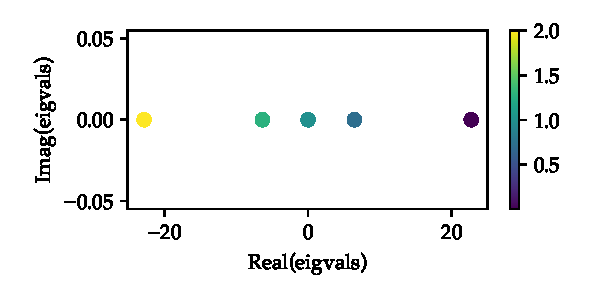
\includegraphics[width=0.55\linewidth]{Figures/simple_example_tv.pdf}
    \caption{Graph total variation (pseudocolor scale) of the normalized eigenvectors, as a function of their respective eigenvalues.}
    \label{fig:simple_example_tv}
\end{figure}

\begin{figure}
    \centering
    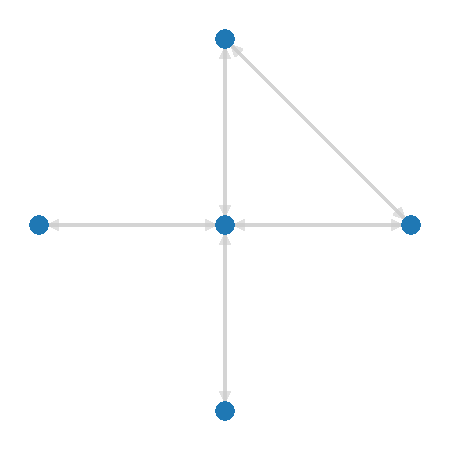
\includegraphics[width=0.3\linewidth]{Figures/degenerate_qgft_graph.pdf}
    \caption{Graph used in the numerical example. The edges are represented by double-headed arrows to indicate the adjacency matrix is not symmetrical.}
    \label{fig:degenerate_qgft_graph}
\end{figure}

\section{Filter design via QLMS optimization}
We have seen so far the establishment of the basis of QGSP, borrowing concepts and tools from GSP and finding the particular consequences of having a quaternion-valued graph shift operator. The last milestone set in the beginning of the last section was to find a method for designing finite impulse response (FIR) LSI filters in QGSP and, fortunately, we can benefit from the large field of adaptive filtering with quaternion signals \cite{ortolani2017frequency}. In this section, we will go through how the quaternion least mean square (QLMS) algorithm can be used for FIR LSI filter design in QGSP, mimicking the method applied in in Subsection \ref{subsec:lsi}.

As the reader may recall, the desired frequency response of the LSI filter with filter taps $\{h_\ell\}_{\ell=0,\dots, L}$ may be defined through a system of linear equations with the format $h(\lambda_i) = \alpha_i$. Using the matrix and vectors
\begin{align}
    \label{eq:siseq2_qgsp_aux}
    \setlength{\arraycolsep}{3pt}
    \underbrace{
        \left[
            \begin{array}{ccccc}
                1 & \lambda_0     & \lambda^2_0     & \dots  & \lambda^L_0     \\
                1 & \lambda_1     & \lambda^2_1     & \dots  & \lambda^L_1     \\
                  & \vdots        &                 & \vdots &                 \\
                1 & \lambda_{N-1} & \lambda^2_{N-1} & \dots  & \lambda^L_{N-1} \\
            \end{array}\right]
    }_{\overset{\Delta}{=} \mathbf{X}}, \quad
    \underbrace{
        \begin{bmatrix}
            h_0    \\
            h_1    \\
            \vdots \\
            h_L
        \end{bmatrix}
    }_{\overset{\Delta}{=} \mathbf{h}}, \quad
    \underbrace{
        \begin{bmatrix}
            \alpha_0 \\
            \alpha_1 \\
            \vdots   \\
            \alpha_{N-1}
        \end{bmatrix}
    }_{\overset{\Delta}{=} \mathbf{y}}
\end{align}
this system of equations can be written in matrix form as
\begin{equation}
    \label{eq:siseq2_qgsp}
    \mathbf{h}^T \mathbf{X}^T = \mathbf{y}^T,
\end{equation}
very similar to (\ref{eq:siseq2}). The odd use of transposition in (\ref{eq:siseq2_qgsp}) is justified by the noncommutativity of quaternion multiplication: the following discussion requires that the filter taps left-multiply the eigenvalues' powers, otherwise the QLMS equations would have different formulations.

Back to the methodology of filter design, after choosing the cutoff frequency (or frequencies) of the ideal filter one wishes to approximate and setting to 1 the values $\alpha_i$ within the passband (zero otherwise),
the intended FIR filter is designed by means of the QLMS algorithm, which was proposed by Took in 2009 \cite{took2008quaternion}. Although many different versions have been formulated since then \cite{ogunfunmi2015adaptive, almeida2014low, ortolani2016quaternion}, all consist in solving the optimization problem
\begin{equation}
    \label{eq:opt}
    \underset{\{\widetilde{h_\ell}\}_{0, \dots, L}}{\text{min}} J(\mathbf{\widetilde{h}}),
\end{equation}
with $\mathbf{\widetilde{h}}$ being an estimation of the desired filter, by means of the LMS-like update rule
\begin{equation}
    \label{eq:updateqlms}
    \mathbf{\widetilde{h}}^{(k+1)} =
    \mathbf{\widetilde{h}}^{(k)} +
    \mu \nabla_{\mathbf{\widetilde{h}}^{(k)}} J(\mathbf{\widetilde{h}}^{(k)}).
\end{equation}

The core difference between QLMS approaches stem from the subjacent definition of $\nabla_{\mathbf{\widetilde{h}}} J(\mathbf{\widetilde{h}})$, the gradient of the real-valued mean squared error cost function $J$ with respect to the quaternion-valued vector $\mathbf{\widetilde{h}}$ (which depends on the concept of quaternion derivatives, a subject matter of many research papers, e.g. \cite{xu2015enabling,jahanchahi2012gradient}). The approach used in this thesis was the original one, from \cite{took2008quaternion}, which considers the following formulation -- adapted to be in matrix form -- for the estimation error and cost function,
\begin{align}
    \label{eq:errorqlms}
    \mathbf{e}(\mathbf{\widetilde{h}}^{(k)}) & \overset{\Delta}{=}
    \mathbf{y} -
    \left( \mathbf{\widetilde{h}}^{{(k)}^T} \mathbf{X}^T \right)^T, \\
    J(\mathbf{\widetilde{h}}^{(k)})          & \overset{\Delta}{=}
    \mathbf{e}^T
    \overline{\mathbf{e}},
\end{align}
in which the notation $\mathbf{e} = \mathbf{e}(\mathbf{\widetilde{h}}^{(k)})$ was used to improve readability. After the gradient derivation in \cite{took2008quaternion}, one arrives at the gradient expression in matrix form
\begin{equation}
    \label{eq:qlmsgradient}
    \nabla_{\mathbf{\widetilde{h}}^{(k)}} J(\mathbf{\widetilde{h}}^{(k)}) =
    2 \left(
    \mathbf{e}^T \overline{\mathbf{X}}
    \right)^T - \mathbf{X}^H \overline{\mathbf{e}}
\end{equation}
providing all that is needed to implement the update rule in (\ref{eq:updateqlms}). The reader is encouraged to refer to \cite{took2008quaternion} and verify the equivalence between the original equations and their matrix forms, just presented. Equations (\ref{eq:updateqlms}) to (\ref{eq:qlmsgradient}) were used exactly as they were written in the computations in Subsection \ref{subsec:denoising}.

As a last and more practical note, it is important to mention that, because of the structure of matrix $\mathbf{X}$, it is indispensable to add the extra step of normalizing the columns of $\mathbf{X}$ before running the QLMS, otherwise convergence is slow, if not even prevented. It is a well known practice for least-mean squares regression and other algorithms based on gradient descent, which do not work well if the features have highly disproportionate scales. Let us recall that this is precisely the current case: the columns in $\mathbf{X}$ represent variables in a regression problem (with target given by the ideal frequency response $\mathbf{y}$) and they differ massively in scale. The normalization here is understood in the sense of bringing the mean and standard deviation of the feature distribution to 0 and 1, respective. That is, for each vector $\mathbf{x}_i = (\lambda^i_0, \lambda^i_1, \dots, \lambda^i_{N-1})^T$ with mean $\mu$ and standard deviation $\sigma$, the normalization takes place by replacing it with $\frac{\mathbf{x}_i - \mu}{\sigma}$.

\section{Examples}

This section is devoted to experimenting with QGSP in real-world datasets, tackling topics such as graph inference, spectral analysis, compression and denoising. All computations in this chapter were performed using \texttt{gspx}, an open-source Python package dedicated to implement the core concepts and tools of QGSP. It constitutes a contribution of this thesis and is available at \url{https://github.com/gboaviagem/gspx}.

\subsection{Denoising a quaternion graph signal via QLMS low-pass filtering}
\label{subsec:denoising}

Let us walk through an example on spectral analysis and denoising. The graph signal will be generated using UK towns' weather data, specifically setting the humidity, atmospheric pressure, temperature and wind speed data to the $1$, $\qi$, $\qj$ and $\qk$ components of each signal sample. The data was fetched from the Open Weather Map API,\footnote{The API is accessible, as of August 2022, at the address \url{https://home.openweathermap.org/}.} in April 20th 2022, at approximately 13:00 GMT, and a sample is shown in Table \ref{tab:02}. The latitude and longitude values of UK towns originate from the LatLong.Net database.\footnote{Accessible, as of August 2022, at the address \url{https://www.latlong.net/category/towns-235-55.html}.}

\begin{figure}
    \centering
    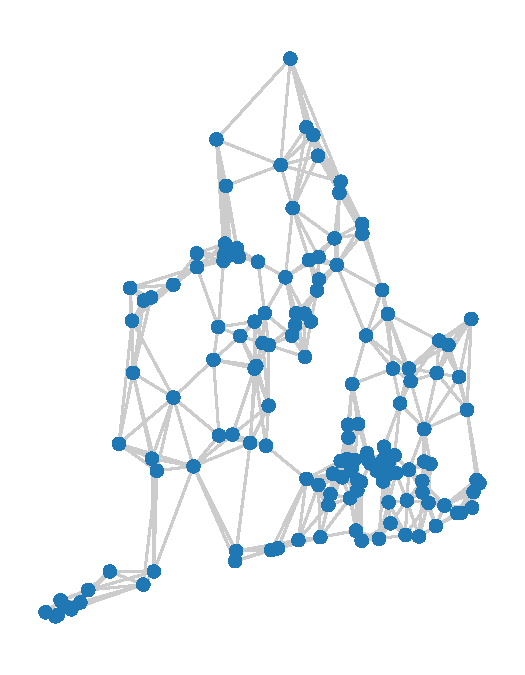
\includegraphics[width=0.3\linewidth]{Figures/uk_example/uk_graph.pdf}
    \caption{Graph created using the 145 towns in England and Wales.}
    \label{fig:uk_graph}
\end{figure}

The graph was created using a nearest-neighbors approach, as in (\ref{eq:weights}), since the nodes possess a clear relation to geographic location. The edge weights were defined using the following steps:
\begin{itemize}[noitemsep]
    \item Compute a real-valued nearest-neighbors adjacency matrix based on the latitude and longitude of UK towns (graph nodes), using the seven closest neighbors to each graph node. At this point, the real-valued edge weights correspond to the euclidian distances between nearby towns \textit{i} and \textit{j}, represented by ${d}(i, j)$.
    \item For each pair of connected nodes from the real-weighted graph in the previous step, compute the \textbf{absolute difference} in \textit{humidity}, \textit{atmospheric pressure}, \textit{temperature} and \textit{wind speed}, represented respectively by ${h}(i, j)$, $p(i, j)$, ${t}(i, j)$ and ${w}(i, j)$. Then, create the quaternion $q(i, j) = {h}(i, j) + \qi {p}(i, j) + \qj {t}(i, j) + \qk {w}(i, j)$ and compute the edge weight
          \begin{equation}
              \label{eq:edge_weight_qgsp}
              \mathbf{A}_{i, j} = \exp^{-1} \left(
              \frac{d(i, j)}{\theta} \cdot
              \frac{q(i, j)}{\parallel q(i, j) \parallel}
              \right).
          \end{equation}
          Finally, in order to exploit the diagonalizability of the adjacency matrix, it was made Hermitian, i.~e., $\mathbf{A}_{i, j} = \overline{\mathbf{A}}_{j, i}$.
\end{itemize}

The reasoning behind the choice of (\ref{eq:edge_weight_qgsp}) is to have edge weights whose magnitude reflect the expected similarity between adjacent signal samples, as in (\ref{eq:weights}), and whose phase are aligned with the difference between such samples. The choice of $\theta$ for the current graph, after some experimentation, was $\theta = 2$.

% Figure \ref{fig:uk_graph} depicts a representation of the UK Town Graph, with quaternion-valued edge weights. A total of 177 towns were used, and the reader may find the full dataset at \url{https://github.com/gboaviagem/gspx/blob/main/resources/uk_weather_at_20Apr202213pm.gz}. The first few rows, so it becomes clear how the data is organized, are displayed in Table \ref{tab:02}.

\begin{table}
    \center
    \captionof{table}{Sample of the dataset containing UK towns' weather data.}
    \label{tab:02}
    \begin{tabular*}{\textwidth}{c @{\extracolsep{\fill}} cccc}
        \toprule
        & \textbf{town} & \textbf{latitude} & \textbf{longitude} & \textbf{humidity (\%)} \\
        \midrule
        1 & St.Asaph & 53.257& -3.442 & 59 \\
        2 & Welling, Bexley&51.45&0.1056&39 \\
        3 & Soham, Ely&52.33&0.3375&43 \\
        4 & Boulmer, Northumberland&55.422&-1.536&79 \\
        5 & Higham Ferrers, East Northamptonshire & 52.303 & -0.592841 & 53 \\
        \midrule
    \end{tabular*}
    \begin{tabular*}{\textwidth}{c @{\extracolsep{\fill}} cccc}
        & \textbf{pressure (hPa)} & \textbf{temp (K)} & \textbf{wind speed (m/s)} & \textbf{wind degrees} \\
        \midrule
        1&1017&288.49&3.71&99 \\
        2&1014&290.09&8.23&80 \\
        3&1016&290.07&6.69&60 \\
        4&1020&282.77&4.07&115 \\
        5&1017&289.78&3.13&53 \\
        \bottomrule
    \end{tabular*}
\end{table}

As a way to remove the scale disparity between the quaternion components (the reader may compare, for instance, pressure and wind speed), each of the 4 columns were linearly scaled down to be within the range $[0, 1]$. A way of visualizing the graph signal is to plot each quaternion dimension separately, as it was done in Fig. \ref{fig:uk_qgsp_graphsig}.

\begin{figure}
    \centering
    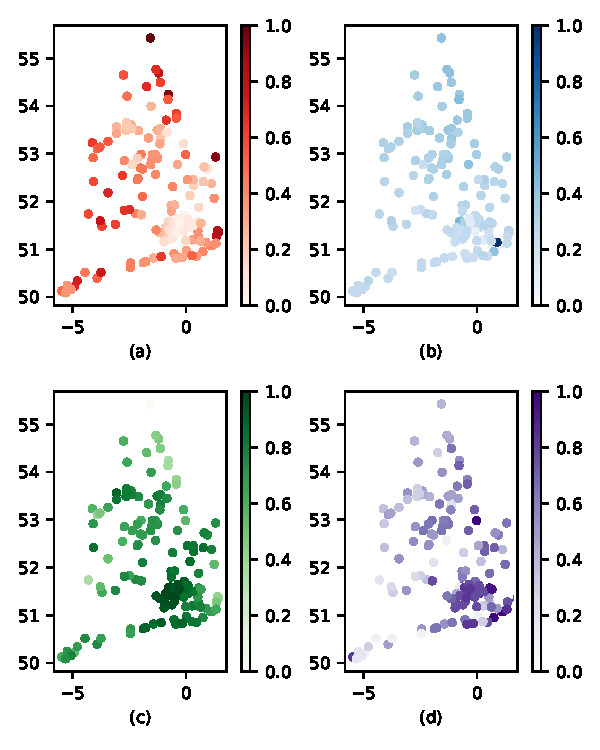
\includegraphics[width=0.55\linewidth]{Figures/uk_signal.pdf}
    \caption{Quaternion graph signal, visualized in the vertex domain. The panels (a) to (d) depict, respectively, the real, $\qi$, $\qj$ and $\qk$ components of each quaternion-valued sample.}
    \label{fig:uk_qgsp_graphsig}
\end{figure}

The QGFT of the graph signal is computed, as defined earlier on this chapter, by the projection of the graph signal on the basis of eigenvectors of the graph adjacency matrix (which is diagonalizable, since it is Hermitian). The signal spectrum is depicted in Fig. \ref{fig:uk_qgsp_spectrum_hermitian}, in which the frequency components are ordered from lowest to highest frequency, using the total variation rule in (\ref{eq:TV_ordering_q}). After the computation of the total variation for each eigenvector, in order to perform the frequency ordering, Fig. \ref{fig:uk_total_variation_hermitian} was generated, demonstrating two previously discussed facts: the eigenvalues of the adjacency matrix are all real-valued and the total variation increases monotonically the further the eigenvalue is from the point $|\lambda_{max}|$ in the complex plane.

\begin{figure}
    \centering
    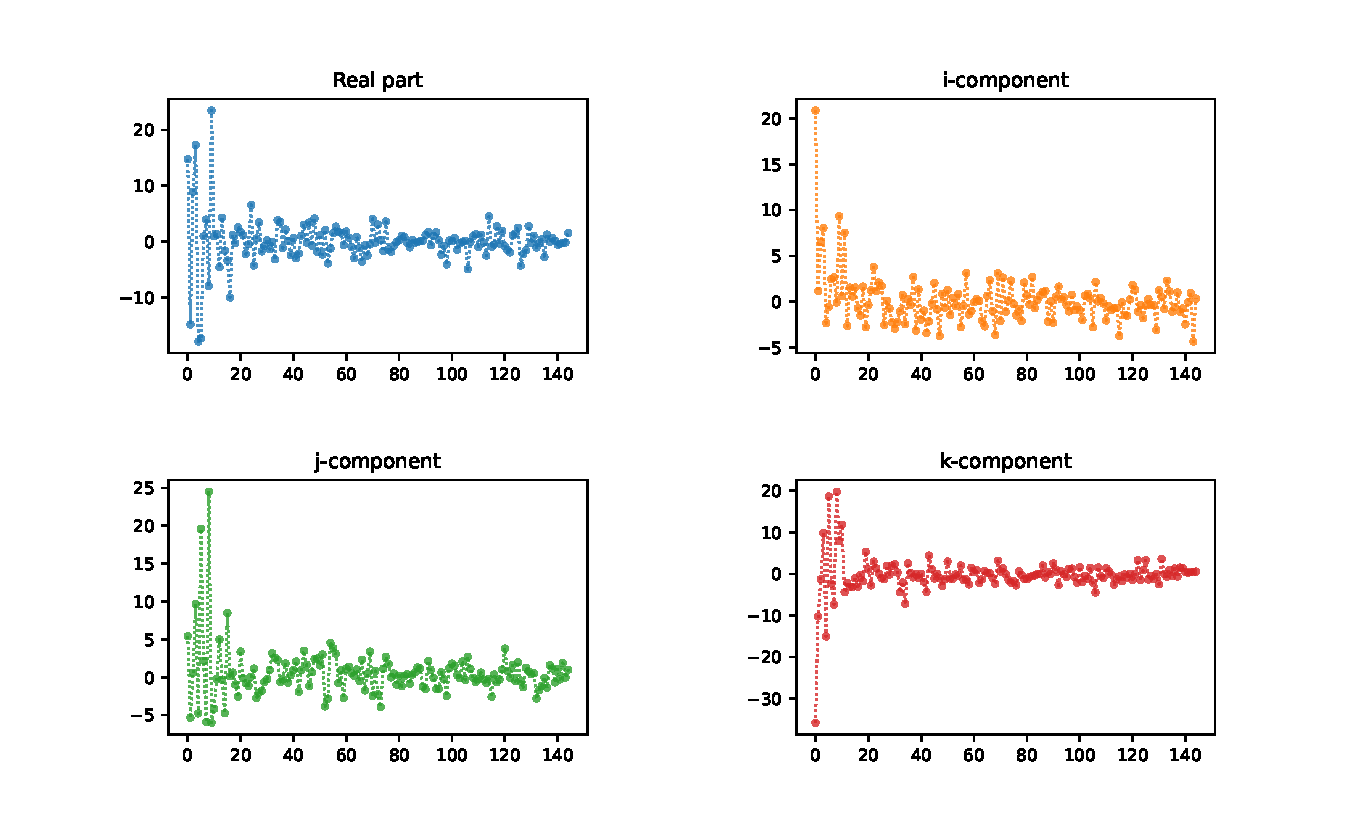
\includegraphics[width=\linewidth]{Figures/uk_example/uk_spectrum_hermitian.pdf}
    \caption{Spectrum of the quaternion graph signal, defined over the vertices of the graph with Hermitian adjacency matrix.}
    \label{fig:uk_qgsp_spectrum_hermitian}
\end{figure}

\begin{figure}
    \centering
    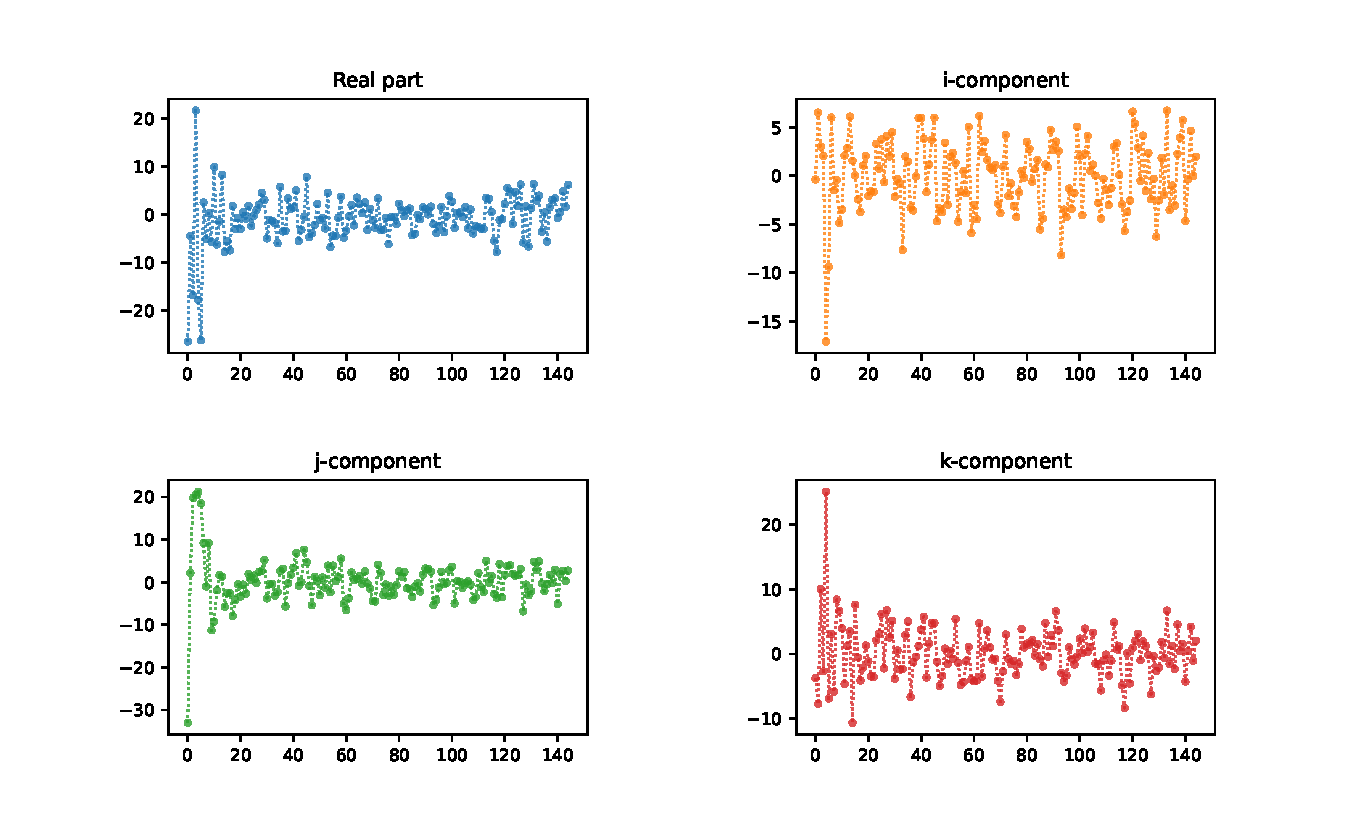
\includegraphics[width=\linewidth]{Figures/uk_example/uk_spectrum_noisy.pdf}
    \caption{Spectrum of the noisy signal.}
    \label{fig:uk_spectrum_noisy}
\end{figure}

Let us now add a white noise on the graph signal, obtained by adding to the original spectrum samples from a uniform distribution with amplitude $5$. The result is shown in Fig. \ref{fig:uk_spectrum_noisy}. The goal of this exercise is to recover as perfectly as possible the original signal out of the noisy one, by using a FIR LSI low-pass filter of length $L+1 = 7$, designed using QLMS.

The ideal low-pass filter was created by setting the passband to have 20\% of the frequency support, i.~e., the values $\alpha_i$ in $h(\lambda_i) = \alpha_i$ were set to 0 except for the eigenvalues corresponding to the 20\% eigenvectors with smallest total variation, in which case $\alpha_i = 1$.

The QLMS algorithm was executed using the following values of step sizes: 0.0001, 0.0005, 0.001 and 0.002, with a maximum of 100 iterations for each step size. To avoid incurring in computational memory overflow, a ``patience'' of 3 iterations were considered, meaning that after 3 iterations of monotonically increasing cost function, the process for that step size was aborted. Any step size greater than 0.002 was found to diverge quickly. Fig. \ref{fig:uk_qlms_iterations} shows the evolution of the cost function during all 100 iterations for each of the mentioned step sizes. The optimal vector $\mathbf{\widetilde{h}}$ was found with $\mu = 0.002$.

\begin{figure}
    \centering
    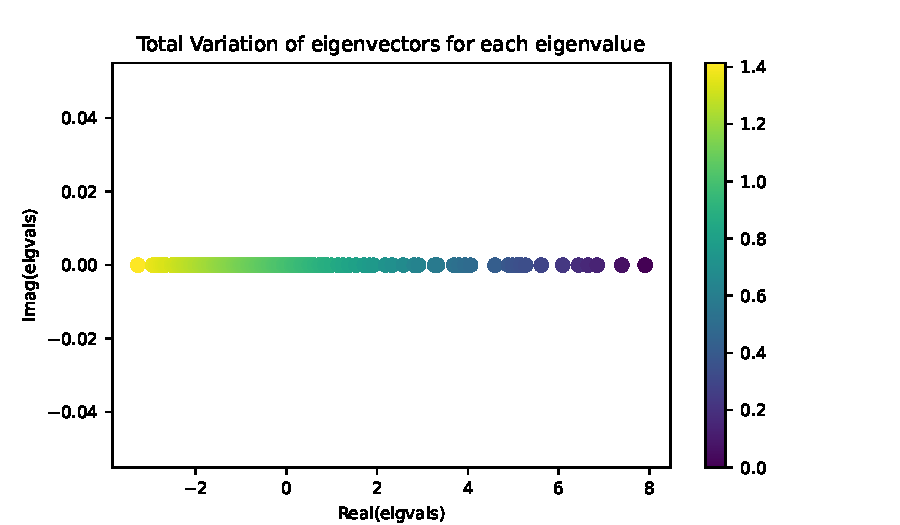
\includegraphics[width=0.65\linewidth]{Figures/uk_example/uk_total_variation_hermitian.pdf}
    \caption{Total variation of the eigenvectors of the Hermitian graph adjacency matrix, for each respective eigenvalue.}
    \label{fig:uk_total_variation_hermitian}
\end{figure}

\begin{figure}
    \centering
    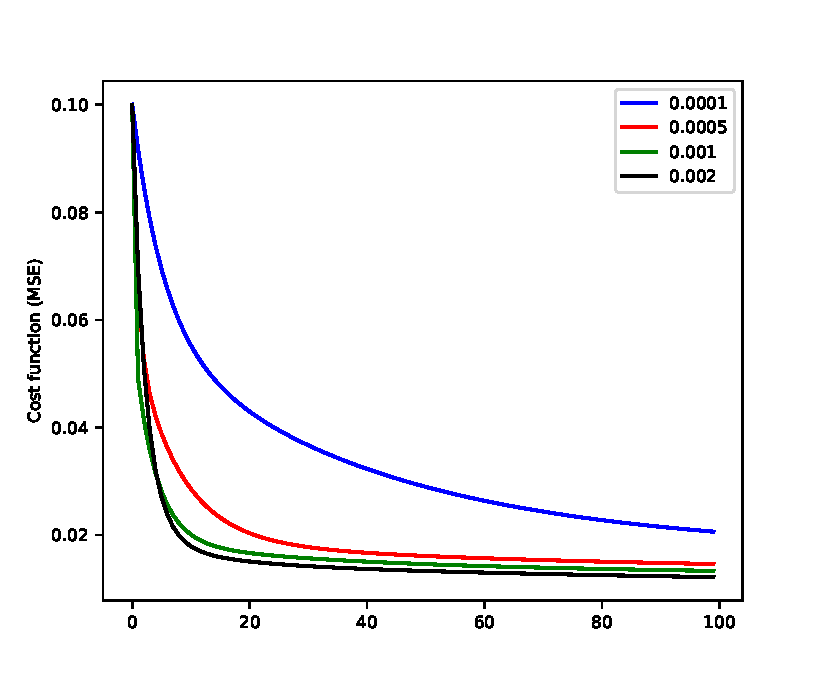
\includegraphics[width=0.65\linewidth]{Figures/uk_example/uk_qlms_iterations.pdf}
    \caption{QLMS cost function for each iteration and for each step size.}
    \label{fig:uk_qlms_iterations}
\end{figure}

The filter taps obtained by the end of the optimization were all real-valued, because the matrix $\mathbf{X}$, the ideal frequency response $\mathbf{y}$ and the vector of initial filter taps (a null vector) are all real-valued: $\mathbf{\widetilde{h}}_{best} = (
    0.199, 0.241, 0.304, -0.177, -0.088, -0.072, 0.014
    )^T$ (rounded up to 3 decimal places).

The frequency response of the FIR low-pass filter which best approximated the ideal one is obtained as in (\ref{eq:siseq2_qgsp}),
\begin{equation}
    \mathbf{y}_{best} = \left(
    \mathbf{\widetilde{h}}_{best}^T \mathbf{X}^T
    \right)^T.
\end{equation}
Fig. \ref{fig:uk_qlm_filter} shows the filter frequency response.

\begin{figure}
    \centering
    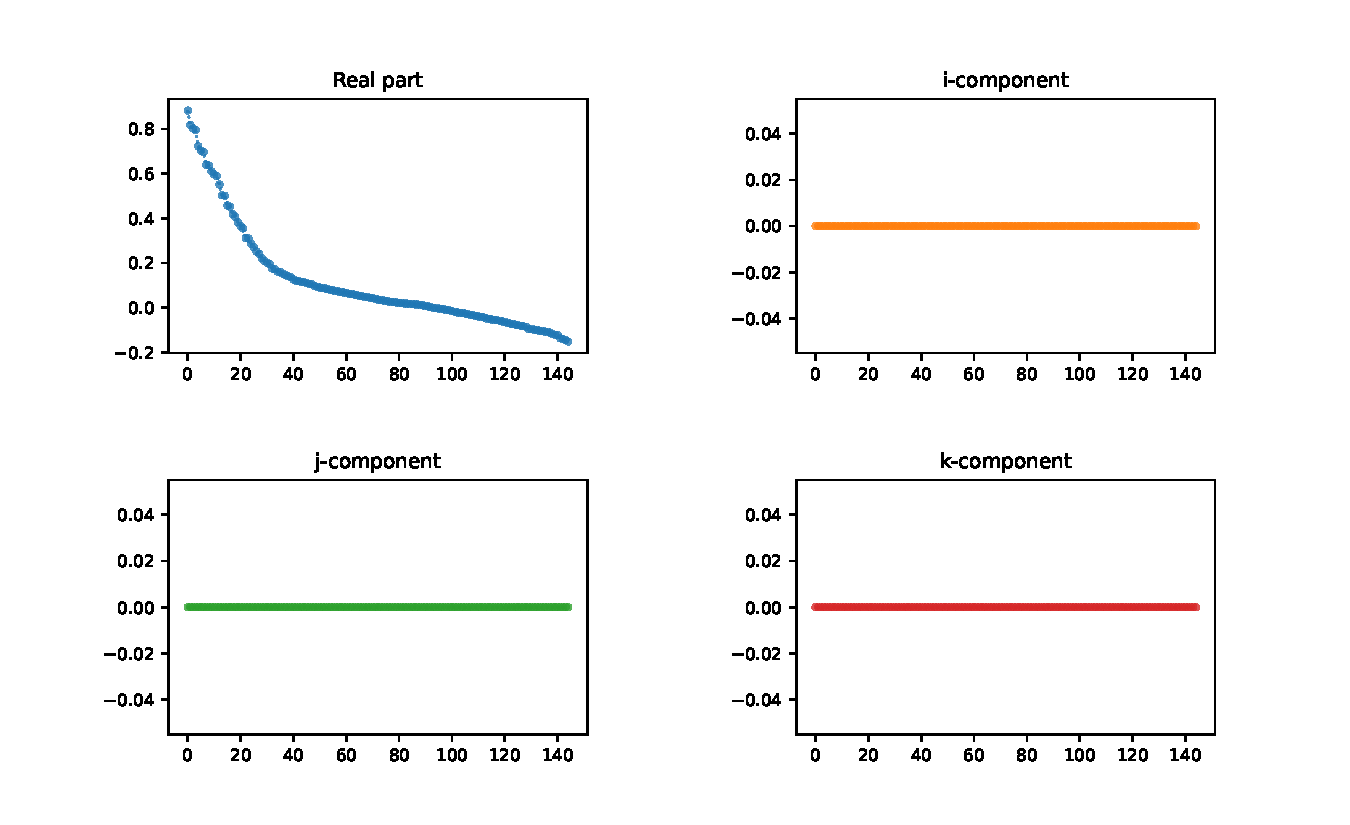
\includegraphics[width=\linewidth]{Figures/uk_example/uk_qlm_filter.pdf}
    \caption{Frequency response of the FIR low-pass filter after running the QLMS.}
    \label{fig:uk_qlm_filter}
\end{figure}

Finally, let us evaluate how well the QLMS filter realizes the denoising in the corrupted signal. As a figure of merit, let us consider the mean squared error between the original $\mathbf{s}$ and filtered $\mathbf{s_f}$ signals, normalized by the total average energy per sample of the original signal. This so called normalized MSE (NMSE) can be written as
\begin{equation}
    \label{eq:errormetric}
    \text{NMSE}\{ \mathbf{s_f} \} \overset{\Delta}{=}
    \frac{\parallel \mathbf{s} - \mathbf{s_f} \parallel}{N}
    \frac{N}{{\parallel \mathbf{s} \parallel}}
    =
    \frac{\parallel \mathbf{s} - \mathbf{s_f} \parallel}{\parallel \mathbf{s} \parallel}.
\end{equation}

Trying out firstly the \textit{ideal} low-pass filter, as a benchmark, we see that it was able to produce a filtered signal with $\text{NMSE}\{ \mathbf{s_{ideal}} \} = 0.166$, dropping by 42\% the error verified in the corrupted signal $\mathbf{s_n}$, which was $\text{NMSE}\{ \mathbf{s_n} \} = 0.28991$. The FIR low-pass filter, designed via QLMS optimization and having only $L+1 = 7$ filter taps, performed better, reaching an error of $\text{NMSE}\{ \mathbf{s_{qlms}} \} = 0.15579$, a 46\% drop. The reason is justified, since the original signal was not null outside the passband, so that the FIR filter was able to preserve more of its energy in that frequency range than the ideal filter.

\subsubsection{Comparison between signal smoothness in symmetric and Hermitian graphs}

The reader may have risen the question of which differences would have appeared if a symmetric adjacency matrix was used, instead of a Hermitian one. Although the graph shift operator would lose the \textit{guaranteed} diagonalizability, the undirect edges would more naturally represent the context at hand, in which similarity between weather in close towns has no directional preference. Let us go briefly through the consequences found when switching from Hermitian to symmetric adjacency matrices.

First of all, it was somehow harder to find a value of $\theta$ in (\ref{eq:edge_weight_qgsp}) which led to a low-pass signal. After some trials, the most satisfactory choice was also $\theta = 2$, but the spectrum profile did not show an energy concentration on low frequencies as good as with the Hermitian case. See Fig. \ref{fig:uk_spectrum_symmetric}.

\begin{figure}
    \centering
    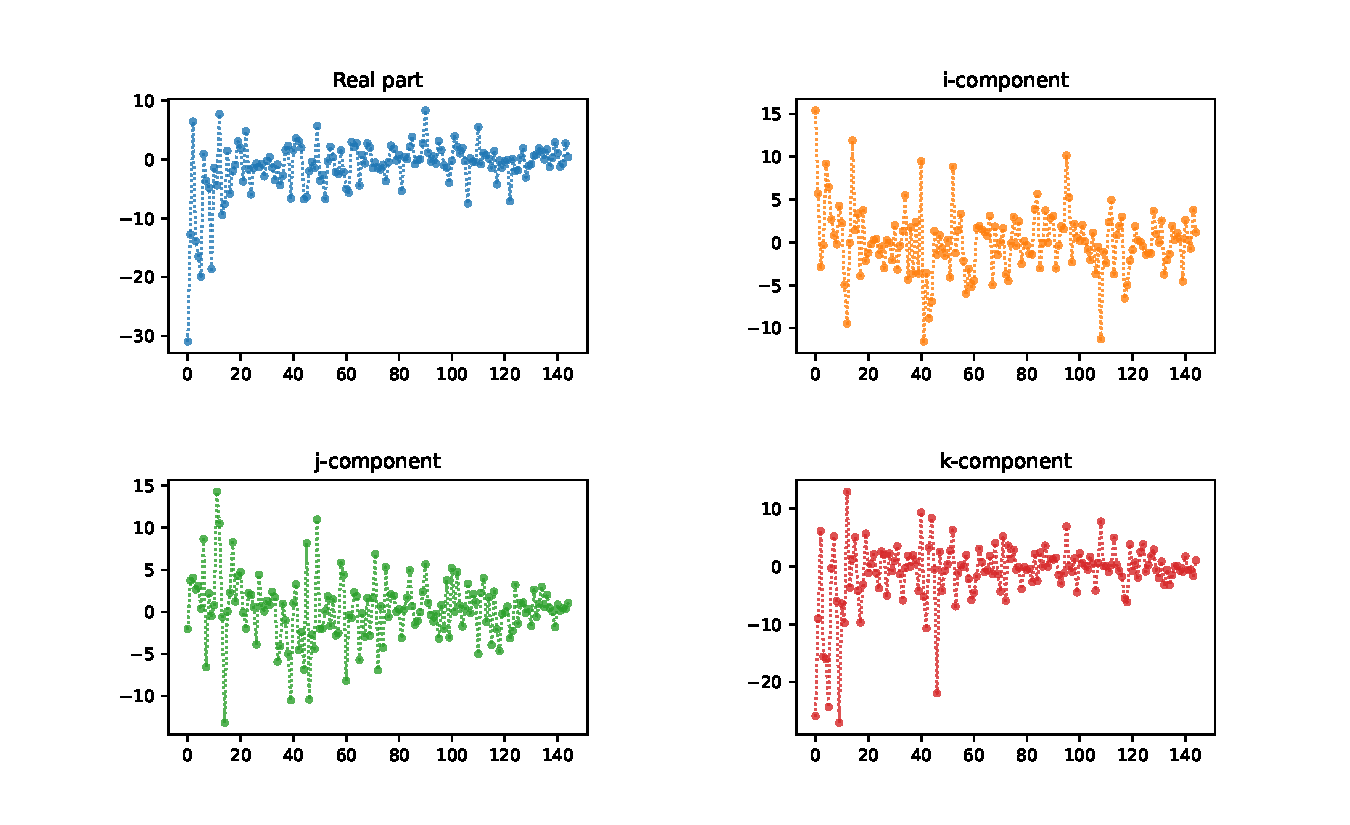
\includegraphics[width=\linewidth]{Figures/uk_example/uk_spectrum_symmetric.pdf}
    \caption{Spectrum of the original signal in the symmetric graph.}
    \label{fig:uk_spectrum_symmetric}
\end{figure}

\begin{figure}
    \centering
    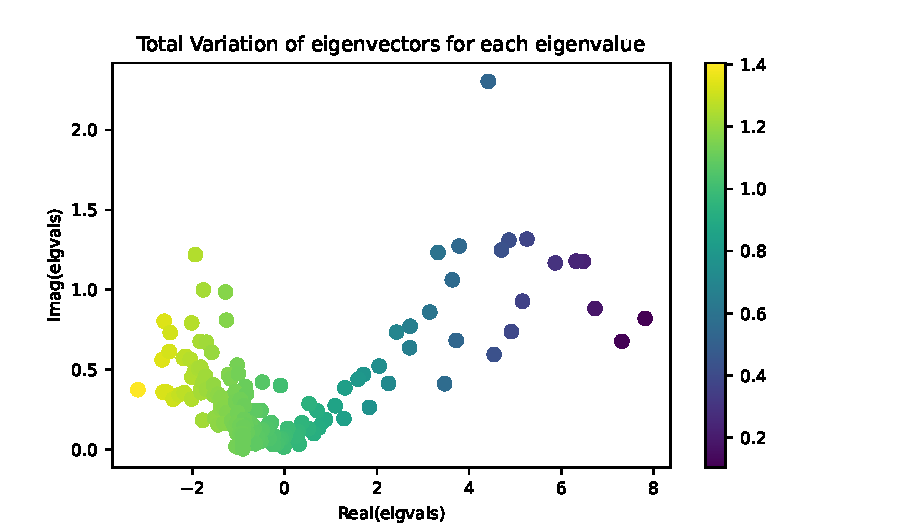
\includegraphics[width=0.7\linewidth]{Figures/uk_example/uk_total_variation_symmetric.pdf}
    \caption{Total variation of eigenvectors of the symmetric graph adjacency matrix.}
    \label{fig:uk_total_variation_symmetric}
\end{figure}

Another difference was the fact that the symmetric quaternion adjacency matrix does not have \textit{only} real-valued eigenvalues. Instead, the standard eigenvalues follow the rule explained in Subsections \ref{subsec:autovetores_XA} and \ref{subsec:eigendecomposition}, being placed either \textit{on} or \textit{above} the real line in the complex plane. See the eigenvalues and the total variation of eigenvectors in Fig. \ref{fig:uk_total_variation_symmetric}.

As a consequence of the eigenvalues being complex-valued, the matrix $\mathbf{X}$ was also complex and the QLMS filter presented a complex frequency response, see Fig. \ref{fig:uk_qlm_filter_symmetric}.
The QLMS algorithm did not suffer, given that the step sizes were conveniently chosen, and converged to the filter taps
\begin{equation}
    \mathbf{\widetilde{h}}_{best} =
    \begin{bmatrix}
        0.199              \\
        0.227 -0.025\qi    \\
        0.148 -0.065 \qi   \\
        -0.062 + 0.002 \qi \\
        -0.031 + 0.049 \qi \\
        -0.030 + 0.037 \qi \\
        -0.016 + 0.020 \qi
    \end{bmatrix}.
\end{equation}
See the cost function \textit{versus} iterations in Fig. \ref{fig:uk_qlms_iterations_symmetric}.


\begin{figure}
    \centering
    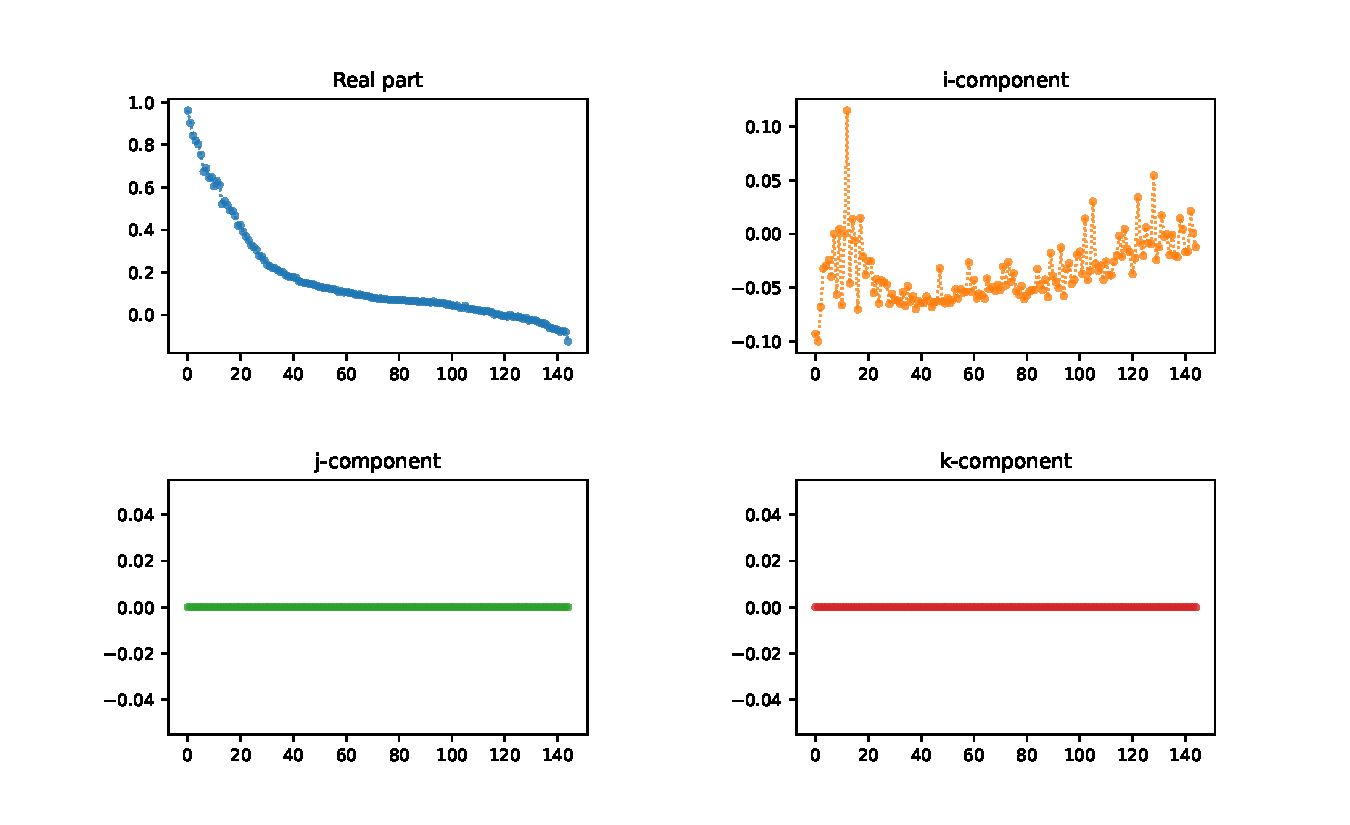
\includegraphics[width=\linewidth]{Figures/uk_example/uk_qlm_filter_symmetric.pdf}
    \caption{Frequency response of the FIR low-pass filter after running the QLMS in the scenario with symmetric graph adjacency matrix.}
    \label{fig:uk_qlm_filter_symmetric}
\end{figure}
\renewcommand{\floatpagefraction}{.9}%
\begin{figure}
    \centering
    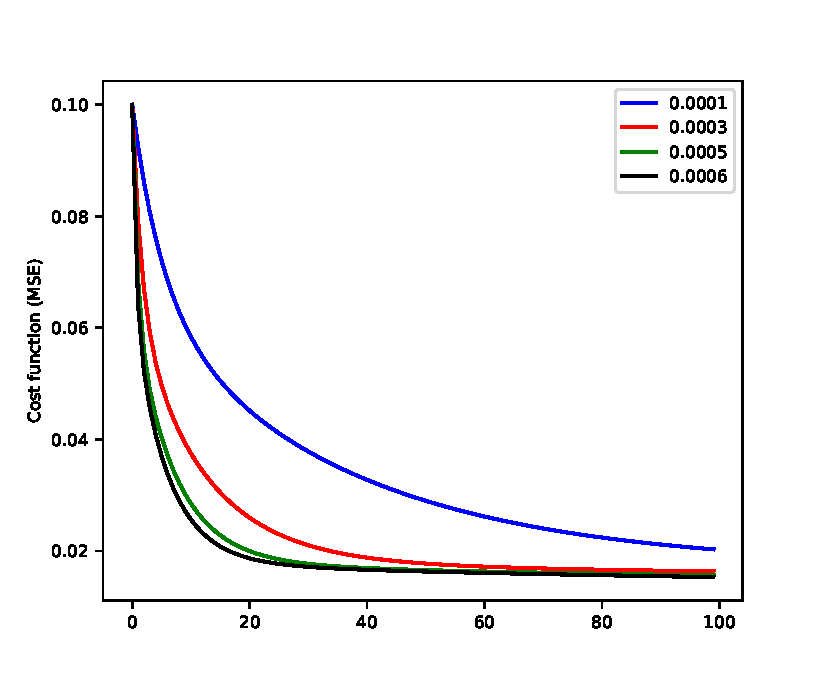
\includegraphics[width=0.58\linewidth]{Figures/uk_example/uk_qlms_iterations_symmetric.pdf}
    \caption{QLMS cost function for each iteration and for each step size, in the scenario with symmetric graph adjacency matrix.}
    \label{fig:uk_qlms_iterations_symmetric}
\end{figure}

\subsection{Spectral analysis and compression of quaternion graph signal}

For this example, let us move away from the UK graph and consider a problem with a larger network. Let us select 1000 of the United States (US) counties and create a simple nearest-neighbors graph out of their geographic coordinates. The resulting undirected graph is depicted in Fig. \ref{fig:us_graph}. It consists of 1000 vertices and 4158 edges. In order to create the quaternion graph signal, four sociodemographic variables will be used. The full source dataset\footnote{Extracted from OpenIntro, a non-profit organization focused on spreading high-quality open-source publications, and avaiable at \url{https://www.openintro.org/data/?data=county_complete}, accessed in October 2022.} comprises 188 variables for each of the 3142 US counties, but only the following indicators were used:
\begin{itemize}[noitemsep]
    \item \textbf{bachelors\_2017}: percent of population that earned a bachelor's degree in 2017.
    \item \textbf{median\_household\_income\_2017}: median household income as of 2017.
    \item \textbf{unemployment\_rate\_2017}: unemployment rate in 2017.
    \item \textbf{uninsured\_2017}: percent of population who were uninsured in 2017.
\end{itemize}
All variables relate to the financial health of american population.

\begin{figure}
    \centering
    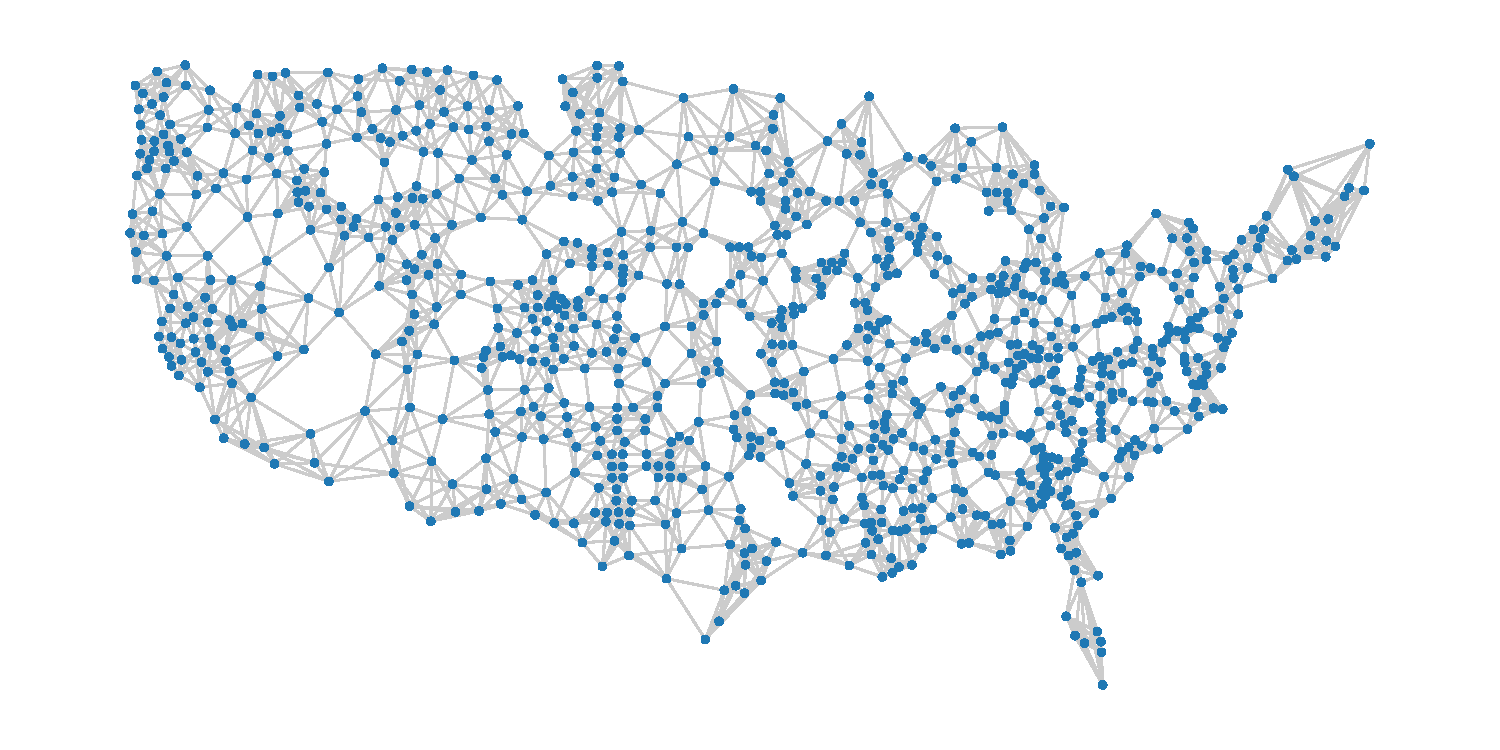
\includegraphics[width=0.8\linewidth]{Figures/usa_example/us_graph.pdf}
    \caption{Nearest-neighbors graph of a few of the United States counties.}
    \label{fig:us_graph}
\end{figure}

Fig. \ref{fig:us_signal} displays each quaternion component as a real-valued graph signal. From the plot (a) to (d), the signals contain the features, respectively: \textit{bachelors\_2017}, \textit{median\_\-household\_\-income\_2017}, \textit{unemployment\_rate\_2017} and \textit{uninsured\_2017}.

\begin{figure}
    \centering
    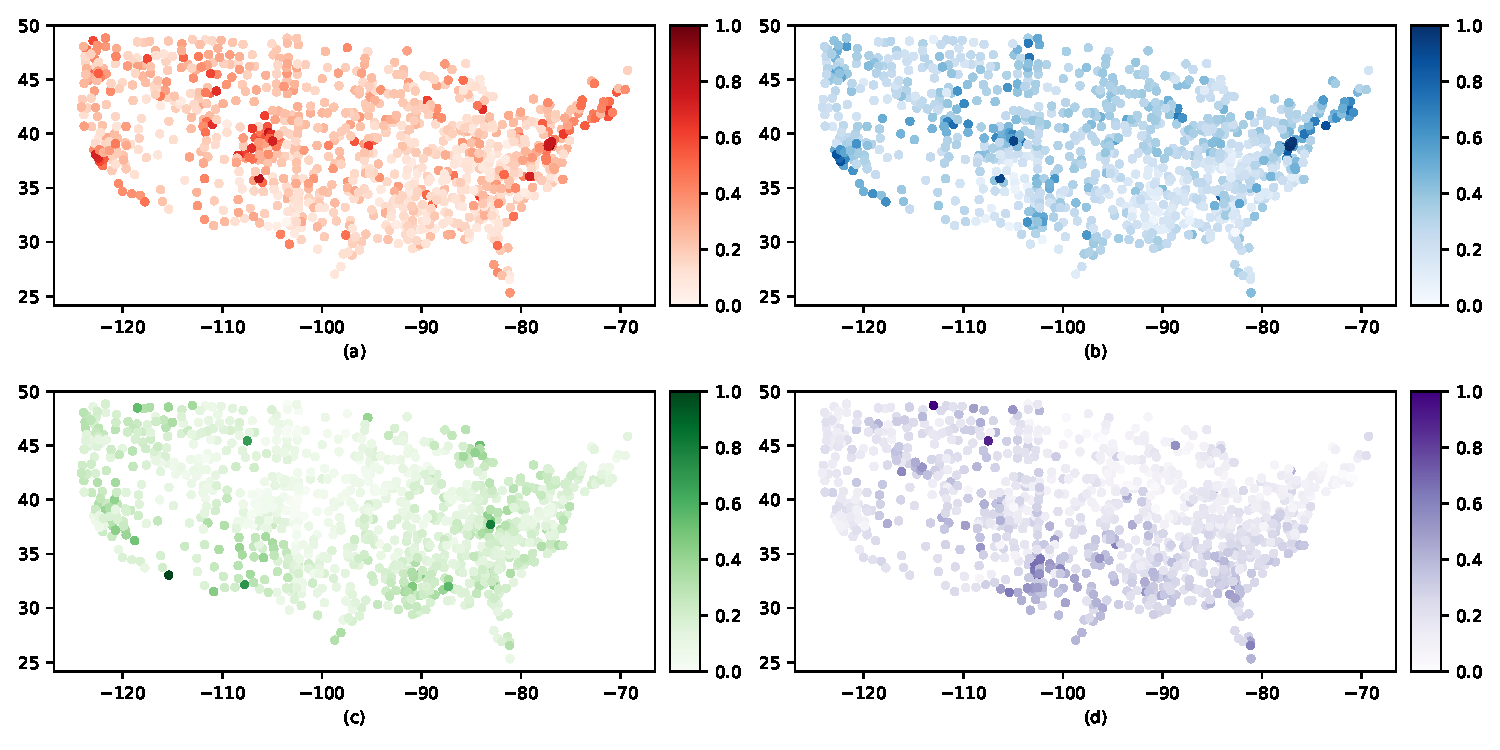
\includegraphics[width=0.95\linewidth]{Figures/usa_example/us_signal.pdf}
    \caption{Sociodemographic quaternion-valued graph signal, split into its components: (a) real part, (b) $\qi$, (c) $\qj$ and (d) $\qk$.}
    \label{fig:us_signal}
\end{figure}

This example is focused on the use of QGSP for compression of multidimensional data. By keeping only a few frequency components with large fraction of the whole signal energy, and given that the underlying graph shift operator is known, the signal representation may be highly condensed. Let us create a Hermitian adjacency matrix, using (\ref{eq:edge_weight_qgsp}) along with the four sociodemographic indicators and the geographic location of each of the 1000 US counties. After the diagonalization of the shift operator the frequency ordering through the total variation metric (see Fig. \ref{fig:us_counties_qgsp_tv1}), the QGFT of the graph signal was computed and is depicted in Fig. \ref{fig:us_counties_qgsp_spectrumsig}.

Before proceeding, however, a few notes regarding the computational challenges of the task must be presented. All calculations were performed (and images were generated) using our \texttt{gspx}\footnote{The library is available as an open repository: \url{https://github.com/gboaviagem/gspx}.} Python package, in a Jupyter Notebook inside a Google Colab Pro instance with 27 GB of RAM. As a representation of the computational cost of computing the QGFT in this 1000-vertices graph, using the mentioned hardware and custom-made code, the time it took to eigendecompose the graph shift operator, sort the frequencies based on total variation and normalize each eigenvector by its L1-norm was roughly around 9 minutes.


\renewcommand{\floatpagefraction}{.8}%
\begin{figure}
    \centering
    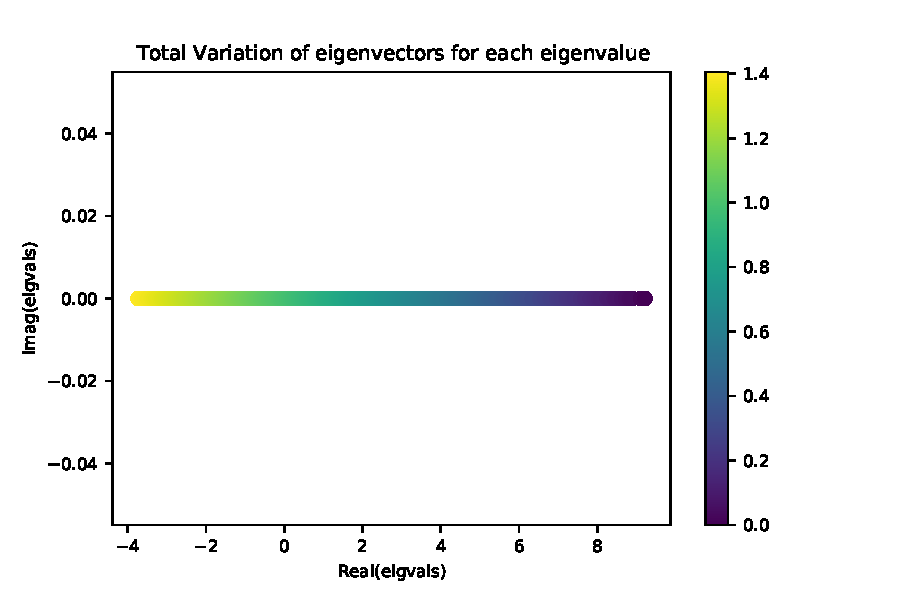
\includegraphics[width=0.65\linewidth]{Figures/usa_example/us_counties_qgsp_tv1.pdf}
    \caption{Total variation for each eigenvector of the (Hermitian) adjacency matrix of the US graph.}
    \label{fig:us_counties_qgsp_tv1}
\end{figure}

\begin{figure}
    \centering
    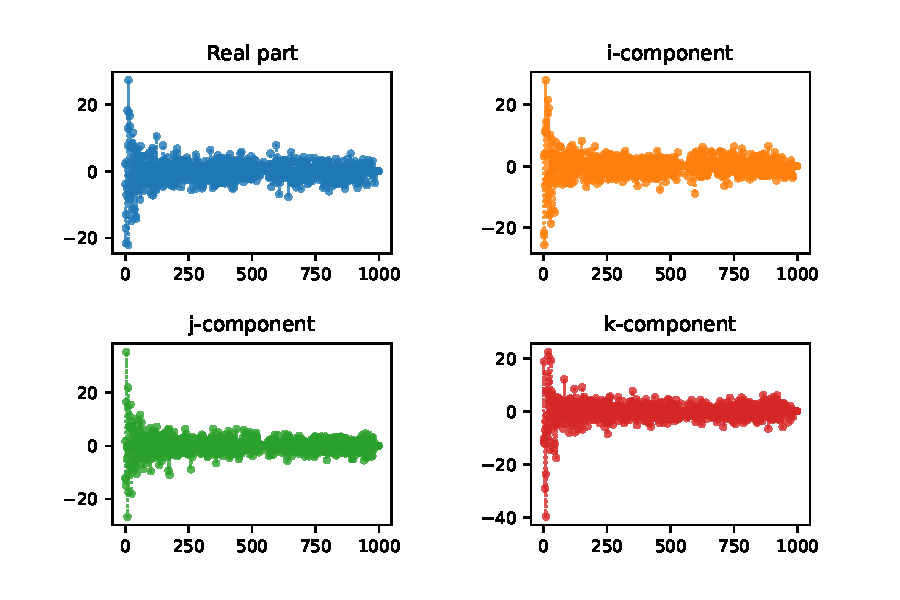
\includegraphics[width=0.95\linewidth]{Figures/usa_example/us_counties_qgsp_spectrumsig.pdf}
    \caption{US graph signal spectrum.}
    \label{fig:us_counties_qgsp_spectrumsig}
\end{figure}

Although the signal presents a heavy noise along all the spectrum, it clearly possesses a prominent low-pass characteristic. Let us measure how well a small fraction of the frequency components with highest energy are able to convey most of the signal.

To this end, 20 values of compression rate were taken, linearly spaced between 5\% and 95\% (inclusive). A compression rate of 5\%, for example, meant that only 5\% of the frequency components with highest energy were kept, the rest being set to zero. After compressing the signal, it was inverse-transformed by the QGFT and compared to the original signal, by means of the same normalized mean squared error used in (\ref{eq:errormetric}).

Fig. \ref{fig:mse_values} shows how the error changed as a function of the compression rate. Since very few frequency components concentrate a relevant amount of energy, a compression rate of 95\% (only 50 components preserved) reaches an NMSE of only 15.4\%. A drop from 95\% to 90\% in the compression rate produces a steep decay in the NMSE, which goes to 11.8\%, a result that makes sense for a low-pass signal: with a few more frequency components, a large chunk of the signal energy is captured. As the compression decreases (i.~e., more components of the spectrum are kept) the NMSE reduction becomes less and less significant, because smaller fractions of the energy are added.

\begin{figure}
    \centering
    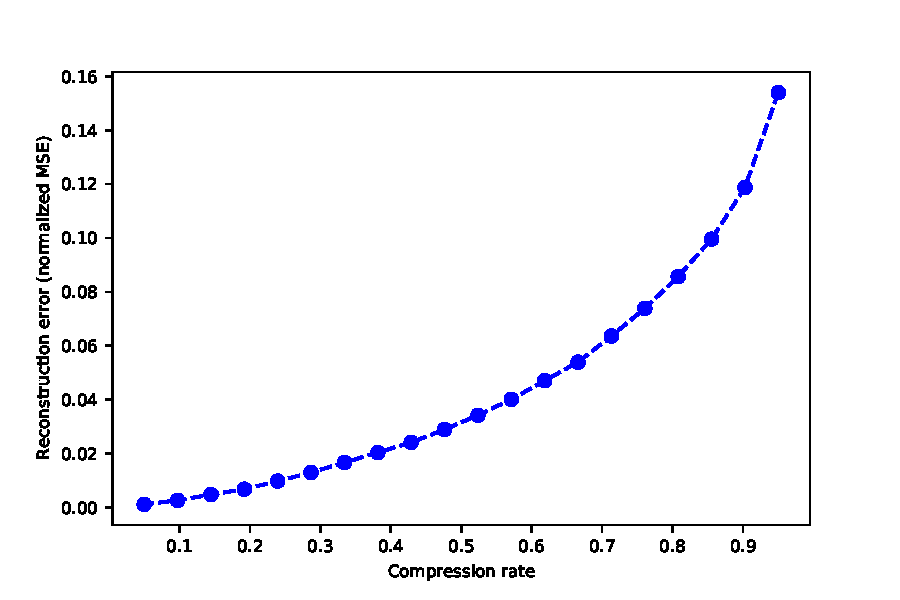
\includegraphics[width=0.7\linewidth]{Figures/usa_example/mse_values.pdf}
    \caption{Normalized mean squared error as a function of the compression rate.}
    \label{fig:mse_values}
\end{figure}

\section{Summary}

We have proposed a new extension of the field of graph signal processing, by pondering the question of (and proposing) how to perform signal analysis and filtering on quaternion-valued signals defined on graphs with quaternion-valued edge weights. By sewing together tools and concepts from quaternion algebra, quaternion adaptive filtering and graph signal processing, the foundations for handling holistically 4-dimensional graph signals were laid. Besides presenting the core definitions of frequency ordering and Fourier transform,
it was presented a condition under which a graph's (quaternion) adjacency matrix is diagonalizable and has unitary eigenvector matrix. Extensive examples with two real-world datasets also illustrate spectral analysis, compression and denoising with QLMS low-pass filters.
